\section{Axiomatic Mathematical Framework}

To isolate malicious behavioral tracking without processing empirical textual histories, the system establishes three foundational axioms governing human interaction spaces.

\subsection{Axiom A: The Ambient Semantic Baseline}
In any stabilized communication channel, the general population generates conversation that centers around a moving average vector space, defining the \textbf{Ambient Semantic Baseline} $\vec{\mu}_t$ within a specific temporal window $t$.

Let a window contain $N$ messages, where each message token sequence is mapped via a local embedding function $\phi(\text{text}) \to \vec{v} \in \mathbb{R}^d$. The baseline is defined as:
\begin{equation}
\vec{\mu}_t = \frac{1}{N} \sum_{i=1}^{N} \vec{v}_i
\end{equation}

The \textbf{Semantic Divergence ($D_s$)} of an incoming text block vector $\vec{v}_k$ relative to the baseline evaluates the deliberate intent to hijack or redirect the ambient social context:
\begin{equation}
D_s(\vec{v}_k, \vec{\mu}_t) = 1 - \frac{\vec{v}_k \cdot \vec{\mu}_t}{\|\vec{v}_k\| \|\vec{\mu}_t\|}
\end{equation}

\subsection{Axiom B: Morphism Directedness and Network Asymmetry}
We frame the communication network as a Category $\mathbf{C}$ where objects $\text{Ob}(\mathbf{C})$ are network participants, and morphisms $\text{Hom}(A, B)$ are directed text-vector communications from node $A$ to node $B$.

\begin{figure}[h]
\centering
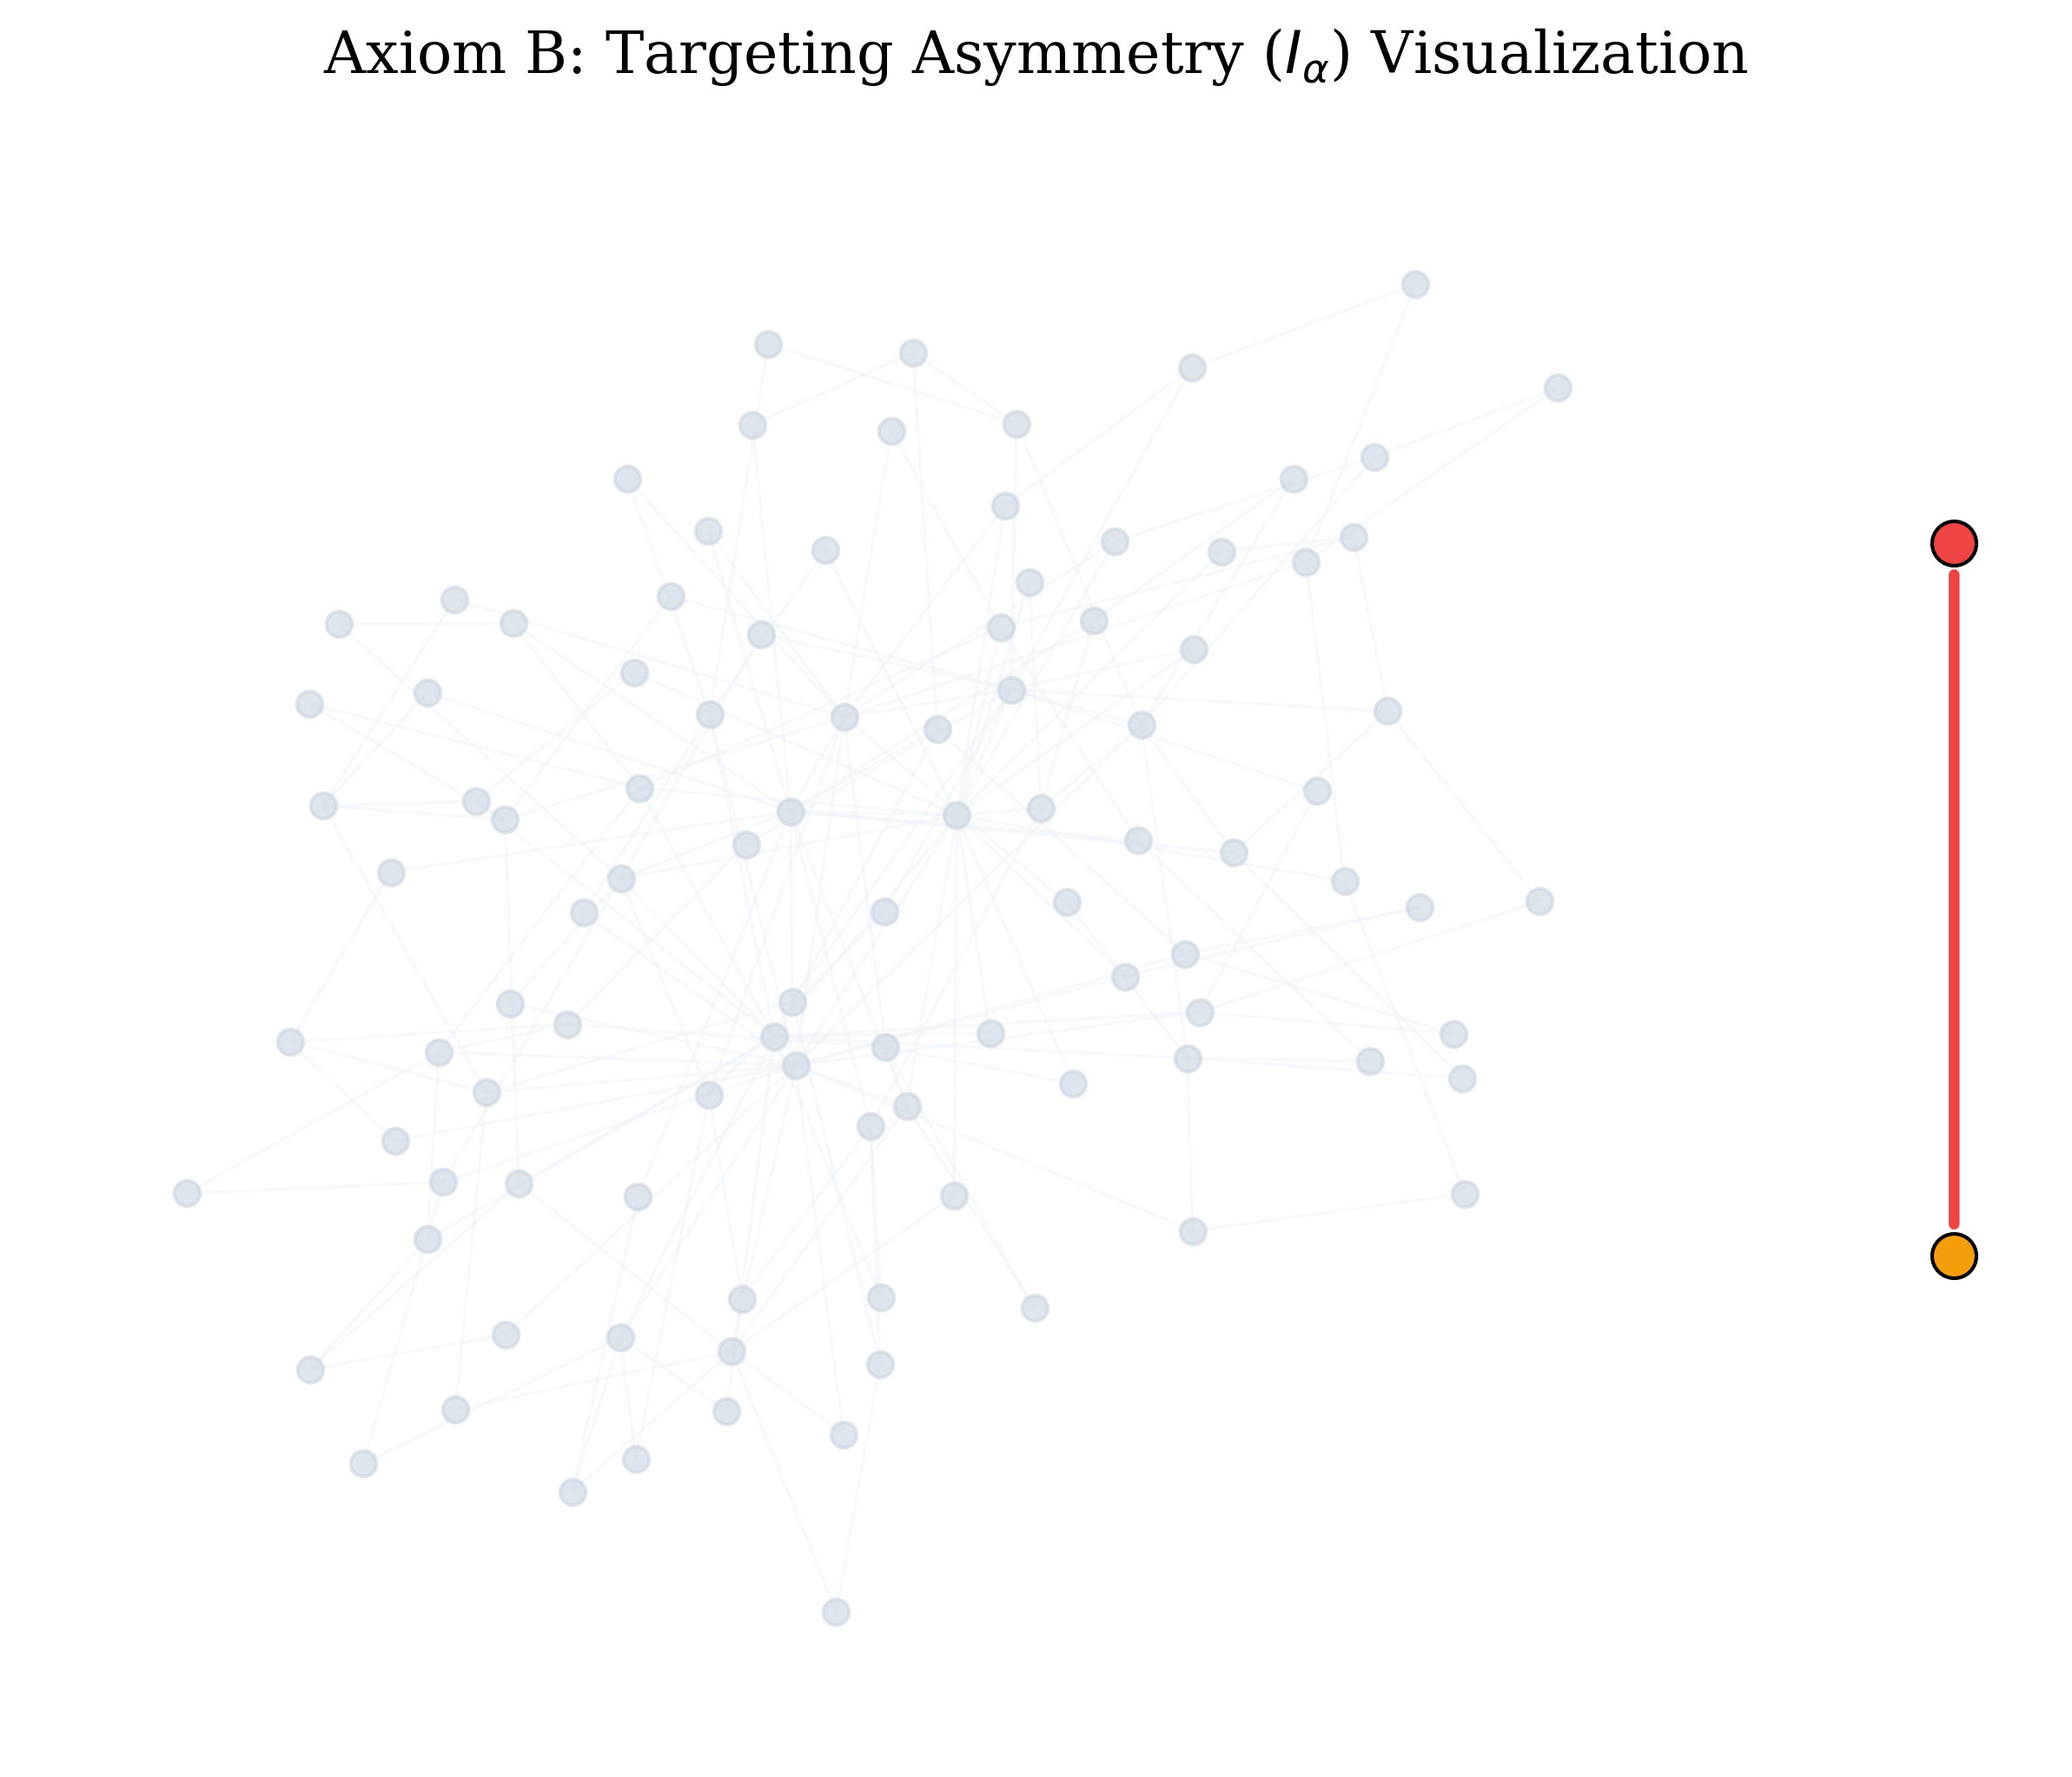
\includegraphics[width=\columnwidth]{../assets/topology_anomaly.png}
\caption{Intense asymmetrical targeting isolating a single node against an ambient background manifold.}
\end{figure}

We define the \textbf{Targeting Asymmetry Index ($I_\alpha$)} for a specific node $A$ over a historical horizon as the ratio of outbound structural intensity directed at a single target node $B$ relative to inbound structural reciprocity:
\begin{equation}
I_\alpha(A \to B) = \frac{\sum \text{Outbound}(A \to B)}{\sum \text{Inbound}(B \to A) + \epsilon}
\end{equation}
where $\epsilon$ is a smoothing parameter minimizing division-by-zero errors.

\subsection{Axiom C: Semantic Velocity and Acceleration Gradients}
Let the semantic vector of a sequence of interactions from node $A$ to node $B$ at sequential timestamps $t_1, \dots, t_n$ be denoted as $\vec{v}_{AB}(t)$. The \textbf{Semantic Velocity ($\vec{V}_s$)} and \textbf{Acceleration ($\vec{A}_s$)} are:
\begin{equation}
\vec{V}_s = \frac{\Delta \vec{v}_{AB}}{\Delta t}, \quad \vec{A}_s = \frac{\partial^2 \vec{v}_{AB}}{\partial t^2}
\end{equation}
A severe negative drop in vector similarity across an exceptionally tight temporal delta signals a hostile context jump.
